\addcontentsline{toc}{chapter}{概要}
\chapter*{概要}

やかんに火をかけて, 湯を沸かすときのことを考えてほしい. やかんのフタには蒸気を逃すために穴が空いているが, それを塞ぐと, やかんの底よりも冷たいフタの裏に細かい水滴が付き, ある程度集まって塊となったらその水滴がポチャンと落ちる様子が想像できるだろう.
先行研究によれば, フタの裏が強く濡れ性(親水性)を持っていると, 流体系は非定常で周期的なダイナミクスを示す.
それは, 「フタの裏付近での水蒸気形成, フタへの水の吸着, そして水の落下」を繰り返すというものである. 
本研究では, 内部の水がフタの裏に引っ付いたり, 落ちたりということを繰り返すことに対して興味を持ち, 数値実験を用いて, その繰り返しに周期性があるか, そのフタの性質によって繰り返しの仕方に変化が生まれるかを調べた. 


\begin{wrapfigure}[12]{R}[5mm]{80mm}
    \centering
    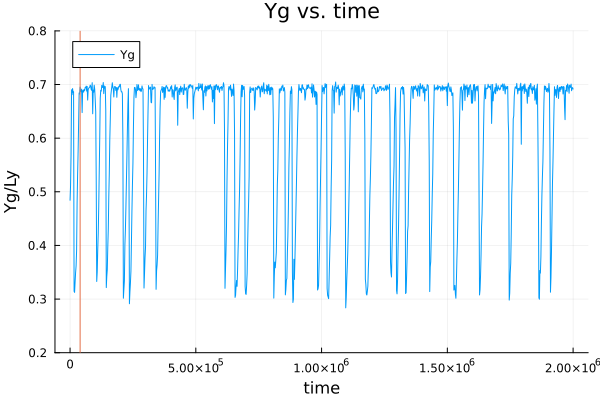
\includegraphics[keepaspectratio,width=80mm]{/Users/2023_2gou/Desktop/r_yamamoto/Report/image/RaRtmap10_cycle/2023-12-28T12:38:52.986_map_10times_chi1.265_Ay50_rho0.4_T0.43_dT0.04_Rd0.0_Rt0.5_Ra1.877538_g0.0003999718779659611_run4.0e8.png}
    \caption{}
    \label{fig: cycle}
\end{wrapfigure}


具体的には, 上下に濡れた壁がつき, 下向きに重力がかかり, 温度差をつけた熱浴を上下に設定することで, 上向きに熱流を流すことを考えた流体系を設計した. 
(ただし, 重力の強さと熱流の大きさを特徴づけるパラメータ $mgL_y$ と $k_{\text{B}}\Delta T$ の比を1程度としている. )
壁の濡れ性をパラメータ制御して, 分子動力学計算を用いて数値実験を行い, 系の重心位置と空間的なばらつきに焦点を当てて分析すると, 周期的なダイナミクスがはっきりと現れる系では, 両者は相空間上で比較的安定した半円の閉軌道を描くことが分かった.$(図\ref{fig: cycle})$
さらに, 壁の濡れ性を強くしたときに, 周期的なダイナミクスがより顕著に現れることも明らかになった. 
